\newpage
\appendix
\FloatBarrier
\section{Figures}
\begin{figure}[!ht]
	\begin{center}
		\includegraphics[width=0.7\textheight]{technologies.png}
		\caption{Basic technology stack}
		\label{technologies}
	\end{center}
\end{figure}

\begin{figure}[!ht]
	\begin{center}
		\includegraphics[width=0.7\textheight]{dataModel.png}
		\caption{Data model}
		\label{dataModel}
	\end{center}
\end{figure}

\begin{figure}[!ht]
	\begin{center}
		\includegraphics[width=0.7\textheight]{components.png}
		\caption{Components}
		\label{components}
	\end{center}
\end{figure}

\begin{figure}[!ht]
	\begin{center}
		\includegraphics[width=0.7\textheight]{chatCommunication.png}
		\caption{Chat Communication Flow}
		\label{chatCommunication}
	\end{center}
\end{figure}

\begin{figure}[!ht]
	\begin{center}
		\includegraphics[width=0.7\textheight]{authflow.png}
		\caption{Authentication Flow}
		\label{authflow}
	\end{center}
\end{figure}

\begin{figure}[!ht]
	\begin{center}
		\includegraphics[width=0.7\textheight]{redux.png}
		\caption{Redux Flow}
		\label{redux}
	\end{center}
\end{figure}

\begin{figure}[!ht]
	\begin{center}
		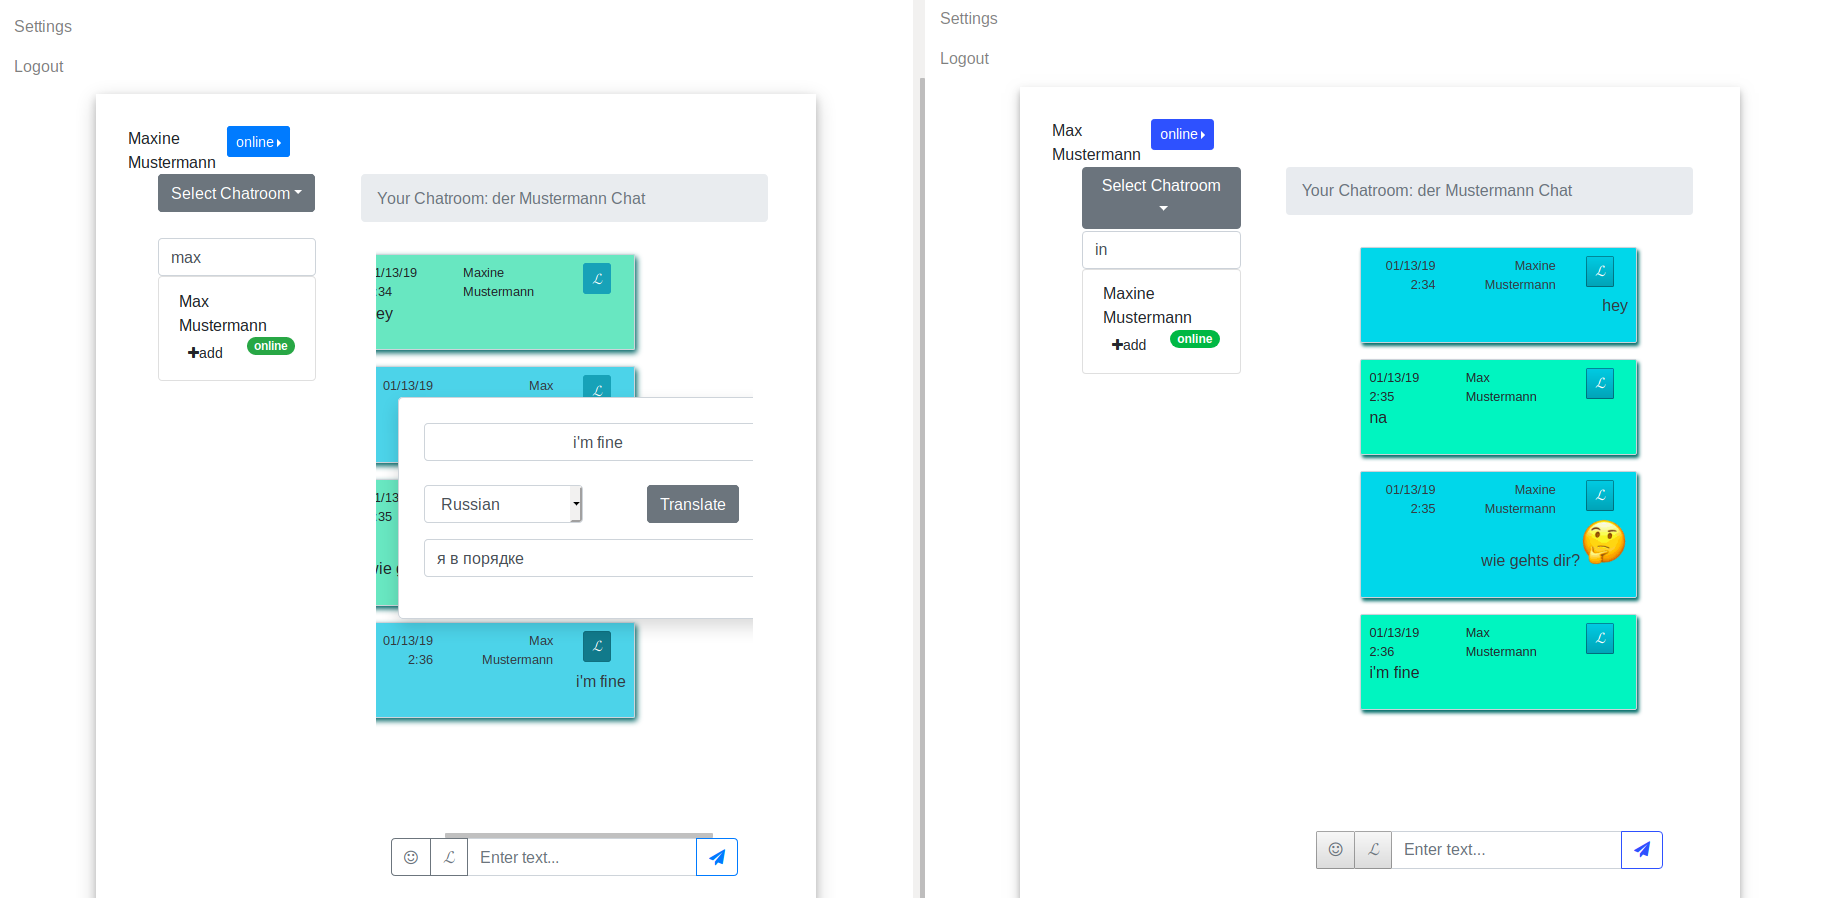
\includegraphics[width=0.7\textheight]{chat.png}
		\caption{Chat room}
		\label{chat}
	\end{center}
\end{figure}

\begin{figure}[!ht]
	\begin{center}
		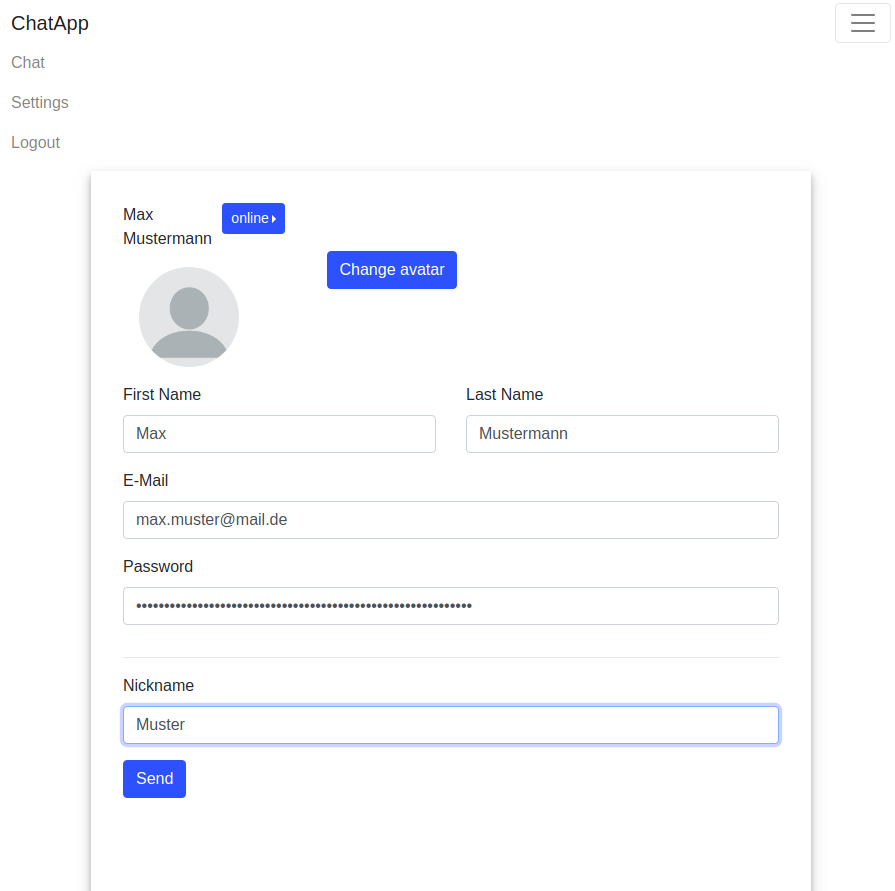
\includegraphics[width=0.7\textheight]{settings.png}
		\caption{User settings}
		\label{settings}
	\end{center}
\end{figure}

\FloatBarrier
\section{Tables}
\noindent
\renewcommand{\arraystretch}{1.5}
\renewcommand{\check}{x}
\FloatBarrier
\begin{table}[!htp]
	\begin{tabularx}{\textwidth}{p{.3\textwidth}XXXX}
		
		& \textbf{Jung} & \textbf{Martensen} & \textbf{Engelmann} & \textbf{Steeg} \\\hline\hline
		Registration & \check & & &  \\ \hline
		Login & \check & \check & \check & \\\hline
		Chatroom creation & & \check & & \\\hline
		Change user settings &  \check & & & \\\hline
		Set online status & \check & \check & & \check\\\hline
		Text translation via yandex & & & \check & \\\hline
		Send/recieve messages & \check & \check & \check & \\\hline
		Initialize/optimize development workflow (docker etc) & \check & & & \\\hline
		Retrieve Chat History & & \check & & \\\hline
		User list & \check & \check & & \check \\\hline
	\end{tabularx}
	\caption{Task assignment for the project}\label{table:task-assignment}
\end{table}

\begin{table}[!htp]
	\begin{tabularx}{\textwidth}{XX}
		\textbf{Status} & \textbf{Feature} \\\hline
		Done & User can register \\
		& User can see chat history \\
		& User can write and send message \\
		& User can create chat rooms \\
		& User can change user preferences \\
		& User can delete his created chat rooms \\
		& User can infite others to chatroom \\
		& User can translate messages \\
		& User can send emojies \\\hline\hline
		Feature Task
		& User can join chatroom on his own \\
		& User can edit messages \\
		& Guest can join chatroom with only reading access \\
		& User can stay logged in with re-entering credentials \\
		& User can see new messages as highlighted \\
		& User can receive recommendation on channels \\
		& User can receive a user rating due to his activity \\
		& User can see the status and their updates of other users \\
		& User can format his messages with newlines \\
		& User can set his avatar
	\end{tabularx}\caption{Feature list for the chat application}\label{fig:feature-list}
\end{table}
